\input{Header.tex}

\begin{document}

%%%%%%%%%%%%%%%%%%%%%%%%%
%		Caratula		%
%%%%%%%%%%%%%%%%%%%%%%%%%

\begin{titlepage}
\newcommand{\HRule}{\rule{\linewidth}{0.5mm}}
\center
\mbox{\textsc{\LARGE \bfseries {Instituto Tecnológico de Buenos Aires}}}\\[1.5cm]
\textsc{\Large 22.05 Análisis de Señales y Sistemas Digitales}\\[0.5cm]


\HRule \\[0.6cm]
{ \Huge \bfseries Trabajo práctico N$^{\circ}$N}\\[0.4cm] 
\HRule \\[1.5cm]


{\large

\emph{Grupo 3}\\
\vspace{3px}

\begin{tabular}{lr} 	
\textsc{Mechoulam}, Alan  &  58438\\
\textsc{Lambertucci}, Guido Enrique  & 58009 \\
\textsc{Rodriguez Turco}, Martín Sebastian  & 56629 \\
\textsc{Londero Bonaparte}, Tomás Guillermo  & 58150 \\
\end{tabular}

\vspace{20px}

\emph{Profesores}\\
Jacoby, Daniel Andres\\
Belaustegui Goitia, Carlos F.\\
Iribarren, Rodrigo Iñaki\\
\vspace{3px}
%\textsc{} \\	

\vspace{100px}

\begin{tabular}{ll}

Presentado: & ??/??/20\\

\end{tabular}

}

\vfill

\end{titlepage}


%%%%%%%%%%%%%%%%%%%%%
%		Indice		%
%%%%%%%%%%%%%%%%%%%%%

\tableofcontents
\newpage

%%%%%%%%%%%%%%%%%%%%%
%		Informe		%
%%%%%%%%%%%%%%%%%%%%%

%\section{Introducción}
%	\label{intro}
%	\input{../Informe/Header.tex}

\begin{document}
\subsection{Implementación por lógica discreta}
Para la lógica combinacional lo primero que se hizo fue escribir las posiciones de memoria en las que vivirá nuestro periférico en binario.
\begin{align}
0x4000 \implies 16384 \implies 0100 0000 0000\\
0x2000 \implies 8192(Memory)\\
0x6000 \implies 24576 \implies 011000000000 
\end{align}
De aqui se arma la tabla de verdad de los últimos 3 bits mas significativos.
\begin{table}[H]
\centering
\begin{tabular}{cccc}
$a_{15}$ & $a_{14}$ & \multicolumn{1}{c|}{$a_{13}$} & CS \\ \hline
0 & 0 & 0 & 0 \\
0 & 0 & 1 & 0 \\
0 & 1 & 0 & 1 \\
0 & 1 & 1 & 1 \\
1 & 0 & 0 & 0 \\
1 & 0 & 1 & 0 \\
1 & 1 & 0 & 0 \\
1 & 1 & 1 & 0
\end{tabular}
\label{tab:truetab}
\end{table}
De aquí se puede solucionar el mapa de karnaugh para la siguiente configuración:
\begin{figure}[H]
  \centering
  \includegraphics[width=0.5\textwidth,page = 1]{ImagenesEjercicio1/Circuits.pdf}
  \caption{Lógica Discreta}.
  \label{fig:circLog}
\end{figure}
\subsection{Implementación por lógica de baja complejidad}
Se utilizó el decodificador 74LS139, conectando a los pines $a_{15}$ y $a_{14}$ a las entradas B y A respectivamente, el CS será la salida $Y_1$ quedando de la siguiente manera
\begin{figure}[H]
  \centering
  \includegraphics[width=0.5\textwidth,page = 2]{ImagenesEjercicio1/Circuits.pdf}
  \caption{Lógica de baja complejidad}.
  \label{fig:circdec}
\end{figure}
\subsection{Implementación por medio de una PAL}
Se utilizó una PAL como decodificador de direcciones,como se observa en la tabla (\ref{tab:truetab}) es posible detectar el perisferico viendo únicamente los bits $a_{15}$ y $a_{14}$ asi se llega a la siguiente ecuación:
\begin{align}
x_1 = a_{15} \ \ \  \  \  \  \  \  \  \ x_2=a_{14} \\
f1=CS \ \ \ f1= \bar{x_1} \  \&  \ x_2
\end{align}

\subsection{Análisis y construcción del diagrama de tiempos}
Se construyó para el microprocesador M68HC11 el diagrama de tiempos para un ciclo de lectura/escritura, usando como ejemplo la posición de memoria \$2345, la cual está dentro de la hipotética región del mapa de memoria donde se aloja la memoria para la cual se diseñó el decodificador anteriormente.

\begin{figure}[H]
  \centering
  \includegraphics[width=\textwidth]{ImagenesEjercicio1/diagtiempos.png}
  \caption{Ciclo de lectura/escritura de \textit{DATA} en la dirección de memoria \textit{\$2345}}.
  \label{diagtiempos}
\end{figure}
 
Para el análisis de tiempos se tiene en cuenta una frecuencia característica de $2 \ MHz$. Dado esto, se obtiene un rise time de las señales de $t_4 = 20 \ ns$ y un periodo entre ciclos de lectura/escritura de $t_1 = 500 \ ns$, por lo que los tiempos en alto y bajo de la señal \textbf{E} de enable serán de $t_3 = 230 ns$ respectivamente. 

\subsubsection{Primera mitad del ciclo de escritura/lectura}

El comienzo del ciclo de lectura o escritura comienza con el flanco descendente de la señal de enable. Un tiempo $t_{26} = 53 \ ns$ después se activa la señal \textbf{AS} de address strobe, lo cual indica que se utilice el bus de address entero para cargar la parte baja y alta de la dirección de memoria en los puertos C y B del M68HC11 respectivamente. Esta señal se desactiva luego de un tiempo $t_{27} = 96 \ ns$ activando el latch que retendrá la parte baja de la dirección de memoria. De esta manera se logra multiplexar la parte baja del bus de address, o puerto C, para leer o escribir datos al igual que retener la parte baja de la dirección del mapa de memoria.

El puerto C tiene la dirección de memoria por un tiempo válido de $t_{t22} = 88 \ ns$ como mínimo y el puerto B por un tiempo de $t_{12} = 94 \ ns$ como mínimo, que corresponde con el flanco ascendente de la señal de enable y marca la mitad del ciclo de lectura/escritura.

\subsubsection{Segunda mitad del ciclo de escritura/lectura} 
\textbf{Lectura:}
En el caso de la lectura, el tiempo de setup para que el periférico coloque el dato a su salida y lo mantenga estable antes del flanco descendente de la señal de enable es de $t_{17} = 30 \ ns$ y debe ser mantenido estable por $t_{18A} = 10 \ ns$ pasado dicho flanco. Luego pasa a hiZ el puerto C pasados $t_{18B} = 83 \ ns$ de dicho flanco.

\textbf{Escritura:}
Para el caso de la escritura, el puerto C tiene un delay máximo para contener el dato a escribir de $t_{19} = 128 \ ns$ y un tiempo de hold de $t_{21} = 33 \ ns$ como mínimo, por lo cual el tiempo de escritura deberá ser como máximo de $t_{3} + t_{21} - t_{19} = 143 \ ns$.

Finalmente, el address se mantendrá por un tiempo de $t_9$ tras el flanco descendente de la señal de enable, por lo que el tiempo válido de lectura de la dirección de memoria en un ciclo de $t_1 = 500ns$ será de $t_1 - t_{26} + t_{9} = 480 \ ns$.
 
 
 
 
 
 
 
 
 
 
 
 
 
 
 
 
 
 
 
 
 
 
 
 
 
 
 
 
 
 
 
 
%\begin{table}[H]
%\centering
%\begin{tabular}{cccc}
%\hline
%\textbf{A15} & \textbf{A14} & \textbf{A13} & \textbf{CS} \\
%\hline
%0            & 0            & 0            & 0           \\
%0            & 0            & 1            & 0           \\
%\textcolor{red}{0}           & \textcolor{red}{1}            %& \textcolor{red}{0}            & \textcolor{red}{1}           %\\
%\textcolor{red}{0}            & \textcolor{red}{1}            %& \textcolor{red}{1}            & \textcolor{red}{1}           %\\
%1            & 0            & 0            & 0           \\
%1            & 0            & 1            & 0           \\
%1            & 1            & 0            & 0           \\
%1            & 1            & 1            & 0          \\
%\hline
%\end{tabular}
%\end{table}

\end{document}
%
%\section{Implementación}
%	\subsection{Maquina de estados}
%	\label{imp}
%	El programa fue planteado como una maquina de estados, existiendo nueve estados diferentes. A su vez, cada estado es tratado como una FSM más pequeña.

\begin{figure}[H]
\centering
	\includegraphics[width=0.6\textwidth]{ImagenesEjercicio2/fsm.png}
	\caption{FSM del programa.}
	\label{fig:fsm}
\end{figure}

El estado \textbf{IDDLE} es el estado principal por defecto, en el cual se debe ingresar un ID empleando tanto las dos alternativas posibles (mediante encoder o mediante la tarjeta). Al realizar la validación de dicha ID, se pasa al estado \textbf{ASK PIN}.

\begin{figure}[H]
\centering
	\includegraphics[width=0.6\textwidth]{ImagenesEjercicio2/iddle.png}
	\caption{FSM del estado \textbf{IDDLE}.}
	\label{fig:iddle}
\end{figure}

El estado \textbf{ASK PIN} se obtiene el pin de acceso del usuario, que las ser validado se continua al estado de \textbf{ACCES}.

\begin{figure}[H]
\centering
	\includegraphics[width=0.6\textwidth]{ImagenesEjercicio2/askpin.png}
	\caption{FSM del estado \textbf{ASK PIN}.}
	\label{fig:askpin}
\end{figure}

En \textbf{ACCESS} puede retornarse al estado \textbf{IDDLE} (luego de cierto período de inactividad), al acceso de del edificio abriendo la puerta o a un panel de configuración del sistema.

\begin{figure}[H]
\centering
	\includegraphics[width=0.6\textwidth]{ImagenesEjercicio2/access.png}
	\caption{FSM del estado \textbf{ACCESS}.}
	\label{fig:access}
\end{figure}

Dicho panel de configuración se encuentra conformado por dos estados distintos, siendo estos el estado \textbf{BRIGHTNESS} y \textbf{USERS}. El primero permite cambiar el brillo del display empleado, mientras que el segundo otorga ciertas configuraciones diferenciadas.

\begin{figure}[H]
\centering
	\includegraphics[width=0.6\textwidth]{ImagenesEjercicio2/bright.png}
	\caption{FSM del estado \textbf{BRIGHTNESS}.}
	\label{fig:bright}
\end{figure}

Cabe destacar que cualquier usuario puede acceder tanto a la configuración del brillo como de usuarios, pero dentro de este último estado existen ciertas limitaciones.

\begin{figure}[H]
\centering
	\includegraphics[width=0.6\textwidth]{ImagenesEjercicio2/users.png}
	\caption{FSM del estado \textbf{USERS}.}
	\label{fig:users}
\end{figure}

Cualquier persona puede acceder al estado \textbf{CLAVE}, donde puede cambiar su propio pin de seguridad. Pero solo los que cuentan con el rango de administrador son los que tienen acceso a los dos estados restantes. 

\begin{figure}[H]
\centering
	\includegraphics[width=0.6\textwidth]{ImagenesEjercicio2/clave.png}
	\caption{FSM del estado \textbf{CLAVE}.}
	\label{fig:clave}
\end{figure}

Los estados exclusivos de \textbf{ADD USER} y \textbf{DEL USER} permiten que cualquier administrador agregue a un nuevo usuario o elimine a uno existente respectivamente.

\begin{figure}[H]
\centering
	\includegraphics[width=0.6\textwidth]{ImagenesEjercicio2/adduser.png}
	\caption{FSM del estado \textbf{ADD USER}.}
	\label{fig:adduser}
\end{figure}

\begin{figure}[H]
\centering
	\includegraphics[width=0.6\textwidth]{ImagenesEjercicio2/deluser.png}
	\caption{FSM del estado \textbf{DEL USER}.}
	\label{fig:deluser}
\end{figure}
%	
%	\subsection{Capas e interfaces}
%	\label{drivers}
%	Se separó el programa por capas, siendo la \textbf{App} la principal y subdividiendo la capa de \textbf{Drivers} en las capas de \textbf{HAL} y \textbf{MCAL}. Dicha separación puede verse con detalle en la Figura~(\ref{fig:drivers}), donde se muestra como la \textbf{App} entra en contacto únicamente con los drivers de la placa de desarrollo \textbf{FRDM}, de la \textbf{Placa Verde} y con el \textbf{Lector} de la tarjeta.
 
\begin{figure}[H]
\centering
	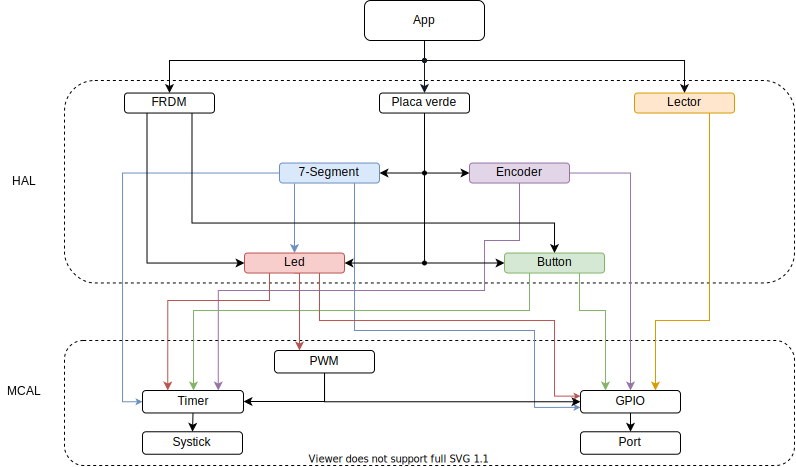
\includegraphics[width=0.9\textwidth]{ImagenesEjercicio3/esquema_drivers.png}
	\caption{Arquitectura del firmware, jerarquía y relación entre los módulos.}
	\label{fig:drivers}
\end{figure}

El driver \textbf{FRDM} emplea los drivers de \textbf{Led} y \textbf{Button}, mientras que la \textbf{Placa Verde}, ademas de los dos recién mencionados, se vale del uso de los drivers de \textbf{Encoder} y del \textbf{7 Segment}. Todos los mencionados junto con el \textbf{Lector} conforman la Hardware Abstraction Layer.

Por otro lado, la Microcontroller Abstraction Layer se encuentra conformada por los drivers de \textbf{Timer}, \textbf{PWM}, \textbf{Gpio}, \textbf{FTM}, \textbf{Systick} y \textbf{Port}, siendo estos últimos 3 los únicos que no tienen contacto con drivers de la HAL. 

En la Figura~(\ref{fig:drivers}) se puede apreciar la interconexión entre drivers de las distintas capas, diferenciando por colores las distintas dependencias entre la HAL y la MCAL para un mejor entendimiento.

\section{OPEN DOOP: Manual de usuario}
	\label{Ejercicio-4}
	\begin{center}
\textcolor{black}{\huge{\textbf{\underline{Manual de usuario}}}}
\end{center}

\begin{center}
\textbf{\LARGE{Inicio:}}
\end{center}

Al encender el dispositivo, se esperará que se ingrese un ID (8 dígitos), utilizando el encoder (rotandolo para seleccionar los números y con el botón del mismo validando el caracter) ó la tarjeta. En caso de que la ID introducida no sea correcta titilará el led \textcolor{red}{rojo} de la FRDM. Una vez ingresada la ID, titilará el led \textcolor{blue}{azul} y deberá ingresar el PIN (5 dígitos). Con el botón del \textbf{CANCEL} (SW2) se puede cancelar la introducción del PIN/ID, mientras que con el \textbf{BACK} (SW3) se vuelve al anterior.

Se cuenta con 3 intentos para ingresar dicho pin. En el caso de que el introducido no sea correcto titilará el led \textcolor{red}{rojo}. Luego de los 3 intentos fallidos, se bloqueará dicho ID, hasta que un \textbf{ADMIN} lo añada de vuelta.

En el caso de inactividad, es decir, que no se efectúe ninguna acción, se volverá al menú de inicio automáticamente, deslogueando al usuario, sin importar en que submenú se encuentre el usuario.

\begin{center}
\textbf{\LARGE{Access:}}
\end{center}

Una vez dentro es posible navegar a través de las distintas opciones mediante el uso del encoder. Las opciones disponibles son ``OPEN'', ``USERS'' y ``BRIGHT''. Open permite abrir la puerta durante 5 segundos. En este intervalo titilará el led \textcolor{green}{verde} y aparecerá un mensaje de ``OPEN DOOR'' en el display. Por otro lado, las otras dos opciones permiten configurar el sistema.

\begin{center}
\textbf{\LARGE{Menúes:}}
\end{center}

\textbf{\Large{Brightness:}}


Permite configurar el nivel de brillo del display, existiendo 3 distintos niveles.

\vspace*{0.5cm}

\textbf{\Large{Users:}}

En este puede configurarse 3 opciones distintas, de las cuales dos son exclusivas para administradores.

\vspace*{0.25cm}
\textbf{\large{Clave:}}
En este submenu, disponible para cualquier usuario, permite cambiar el PIN de seguridad del usuario. Este debe introducirse mediante el uso del encoder.

\vspace*{0.25cm}
\textbf{\large{Delete:}}
\textbf{SOLO PARA ADMINS.} Se muestran en pantalla los distintos ID's disponibles en la base de datos. Gire para cambiar de ID y presione para eliminar.

\vspace*{0.25cm}
\textbf{\large{Add:}}
\textbf{SOLO PARA ADMINS.} En este submenu permite agregar usuarios nuevos a la base de datos, usando tanto el encoder como la tarjeta para agregar el ID pero solo el primero para agregar el PIN.

\begin{center}
\textbf{\LARGE{Consideraciones:}}
\end{center}

El sistema se alimenta con $3.3 \ V$.

\begin{center}
\textcolor{red}{\LARGE{Se debe agregar un pin de testeo (TP) que se encienda mientras se ejecutan las interrupciones, a fin de medir el tiempo que se emplea en la ISR y cuánto representa porcentualmente.}}
\end{center}


\end{document}